% Chapter 2

\chapter{Background} % Main chapter title
This chapter covers in more detail the fundamental concepts needed to assure a
thorough comprehension of the topics discussed in the following chapters.
We start by giving a definition of machine learning, analysing the 
principal aspects of the general approach such as risk minimization and evaluation
strategy.
Then Section \ref{sec:kernel} deals with the theoretical foundations of the 
methods that are in the scope of this thesis, while Section \ref{sec:graphkernels}
delves in the details of the various approaches that are here covered.
Unless otherwise noted, the material in this chapter has been derived
from \cite{nnavarin, rtesselli}.

\label{Chapter2} % For referencing the chapter elsewhere, use \ref{Chapter2} 

\section{Machine learning}

Machine learning is the Artificial Intelligence branch discipline that aims
to approximate human learning processes, which are still rather obscure,
by the means of algorithms and formal methods.
Central to this discipline is the idea of learning a \emph{concept}, or a function
$c(x_i)$ on some example data $x_i \in X$, where the learning process consists
mainly in finding an approximation good enough for the task at hand.
The learning process is carried on by an algorithm which builds an hypothesis
on the available data and uses that hypothesis, let's say $h()$,  to approximate
$c()$.
One of the main goals of such an algorithm is to use the given data to constantly
improve the hypothesis $h()$ up to a certain performance measure, depending
on the task, the paradigm considered or other external factors such as available
resources.

This approach is better exploited in scenarios where either an exact
algorithmic solution to the problem (learning $c()$) would be infeasible, when
there is too much uncertainty in the data or when the problem definition itself
is too difficult to be formally defined or too vague.
Since a machine learning algorithm is often looking for an approximation of the 
optimal solution, the first problem can be solved settling with a suboptimal
solution that is more easily obtainable; given the iterative fashion in which
the learning progresses, data noise can be recognised and avoided; lastly,
an algorithm that learns from the data can be used to explore a problem in multiple
directions, as is often the case with \emph{data mining} oriented approaches.

One of the most common examples of machine learning applications is the binary
classification (Section \ref{subsec:sup}) of so-called spam emails.
This problem states that an email can either be ``spam'' or not but the definition
of ``being spam'' is not unique or universally accepted, so we need to be guided
in the initial definition by a human counterpart: we submit a set of emails to a
human supervisor that labels them for us; then, from this initial evidence, a
machine learning algorithm tries to ``learn'' this particular concept of spam
and uses this knowledge to label future incoming emails which, if confirmed by the
supervisor, go to increase the knowledge base and possibly meliorate it in
a continuing iterative fashion.

This iterative process of learning from experience, incorporating the new one
as it comes, trying to make better decision based on a performance measure, is
the fundamental scheme behind the learning process in machine learning and can
be summed by the following definition:

\begin{definition}[Learning]
    A computer program is said to learn from experience \emph{E} with
    respect to some class of tasks \emph{T} and performance measure \emph{P},
    if its performance at tasks in \emph{T}, as measured by \emph{P}, improves
    with experience \emph{E} \cite{ML}.
\end{definition}

Learning in this context can be divided in three main paradigms, of which this
thesis covers only the first:
\begin{description}
    \item [Supervised learning:] the function to learn has the shape
    $c: X \to Y$ for some sample data $X$ and some target value $Y$.
    The supervision comes from the fact that the target function values are
    given from above by an ``expert'' and plays an active guidance role throughout
    the whole learning process.
    \item [Unsupervised learning:] in this case no target function values are
        given so the algorithm works ``blindly'' trying to catch patterns or
        regularities coming only from the data itself.
    \item [Reinforcement learning:] this is a form of supervised learning
        where the algorithm gets a reward at each search step, reward that can
        be either positive, negative or null, and tries to find the optimal
        strategy to maximize the total reward.
\end{description}

Another big dichotomy in machine learning is given by the way we acquire the
available data, of which again this thesis covers only the first one:

\begin{description}
    \item [Batch learning:] all the data available for learning is given to the
        algorithm beforehand and it all concur, one way or another, in the
        learning process.
    \item [Online learning:] the data becomes available as it gets produced
        and collected so the algorithm can base its learning process only
        on the currently observed sample.
\end{description}

\subsection{Supervised learning}
\label{subsec:sup}

This work considers supervised learning, where each input example has been
previously labelled and represents the evidence data.
We are then facing a \emph{classification} problem, one in which we need to learn
a decision function that will classify each new sample with the correct label.
In this paradigm we are given a set of tuples (i.e. examples) called \emph{training set}:
$S = \{(x_i, y_i)| i=1,\dots,n\}$ with $x_i \in \mathrm{X}, y_i \in \mathrm{Y}$
where $\mathrm{X}$ is the set of data instances and $\mathrm{Y}$ is the set of
labels.
The set $S$ is governed by an underlying unknown probability distribution $P$ over
$\mathrm{X}$.
Furthermore, the domain of $\mathrm{Y}$ defines the type of classification task
that the algorithm should perform:
\begin{itemize}
    \item $Y = \{\pm{1}\}$: binary classification
    \item $Y = \{1,\dots,n\}$: multi-class classification
    \item $Y = \mathbb{R}$: regression, or the approximation of a real function
\end{itemize}

The current work will focus on the first of the three, in other words we will
try to approximate as tightly as possible the function $c:X\to Y$ with an
hypothesis $h:X\to Y, h\in \mathcal{H}$, where $\mathcal{H}$ is the hypotheses
space that is fixed a priori, setting an inductive bias.
Bias can be introduced either by said choice of the hypotheses space or by the
choice of the learning algorithm and is a guarantee that learning is taking place:
a infinite hypotheses space and an exhaustive search algorithm would render
any learning useless since the algorithm could return an infinite number of
hypothesis from $\mathcal{H}$ that could fit any given data.

\subsection{Overfitting}
The kind of bias that we apply to our learning process affects the resulting
hypothesis in ways that can be counter-productive.
Generally it is assumed that the data in the training set is generated according
to an unknown probability distribution $P$ on $X$.
We aim to find an optimal hypothesis $h^*$ that is, the one that minimizes the
prediction error (often referred to as \emph{risk} or ideal error) which is
defined as:

\[R(h)=\int_{X\times Y} L(h(x),y)~dP(x,y)\]

where $L$ is a loss function; given that $P$ is unknown it follows that also
$R(h)$ for any given $h$ is unknown, we can only give a bound on it and measure
the loss function on the classified data we already have, with the following
formula:

\[R_e(h)=\frac{1}{N} \sum_{(x,y) \in S} L(h(x),y)\]

While minimizing the empirical error $R_e(h)$ might be tempting, doing so will
inevitably tailor our hypothesis to the data we have in our training set which
tells us nothing about the underlying (unknown) distribution $P$ nor about the 
possibly infinite set of data that $h$ might have to classify.
Hence we are not consistently modelling the decision function that we are trying
to learn but just the one that fits the set of samples.
Empirical error minimization alone will eventually result in increasing the ideal
error because one of the effect of the minimization is that $h$ will lack
\emph{generalization}.
This situation is called \emph{overfitting} and it occurs when the either the
hypotheses space is too complex or the model has too many parameters with
respect to the number of samples i.e. we are trying too hard to model the
available data.
The contrary is called \emph{underfitting} and negatively affects the
generalization power of an hypothesis by making it fail to learn much from the
sample data.

\subsection{Structural risk minimization}
\label{subsec:srm}
To avoid the scenarios depicted in the previous section we need a way to determine
how powerful an hypothesis can be, i.e. its expressiveness.
This can be achieved by measuring the complexity of the originating hypotheses space,
using a measure called \emph{Vapnik-Chervonenkis dimension} (VC-dimension).
First we will introduce the concept of shattering of a set $\mathrm{X}$:
\begin{definition}[Shattering]
    $S \subset X$ is shattered by an hypotheses space $\mathcal{H}$ iff
    \[\forall S' \subseteq S, \exists h \in \mathcal{H} s.t. \forall x \in S, h(x)=1 \iff x \in S'\]
\end{definition}
i.e. $\mathcal{H}$ implements all the possible dichotomies of $S$.
Given this definition we can now proceed to define more formally what the
VC-dimension is:
\begin{definition}[VC-dimension]
    The VC-dimension of an hypotheses space $\mathcal{H}$, defined on an sample
    space $\mathrm{X}$, is the cardinality of the largest subset of $\mathrm{X}$
    shattered by $\mathcal{H}$, or:
    \[VC(\mathcal{H}) = \max_{S\subseteq \mathrm{X}} |S| : \mathcal{H}\text{ shatters }S\]
\end{definition}
and indeed $VC(\mathcal{H})=\infty$ if $S$ is infinite.

Now, while referring to a binary classification task as is the scope of the present
work, we can show how the VC-dimension affects the bound on the ideal error:
\begin{displaymath}
    R_D(h_{w^*}(x)) \leq R_e(h_{w^*}(x)) + \sqrt{\frac{VC(\mathcal{H})}{N}
    (\log{(\frac{2N}{VC(\mathcal{H})})}+1) - \frac{1}{N}\log{\delta}}
\end{displaymath}
where $R_D$ is the true risk (i.e. ideal error), $R_e$ is the empirical error,
$h_{w^*}(x)$ is the optimal hypothesis returned by the algorithm and $N$ is the
cardinality of the training set.

As we can see, the first term in the rightmost part of the inequality only 
depends from the hypothesis while the second term depends from the ratio
between the VC-dimension and training set size, beside the confidence ($\delta$)
with which the bound is valid.
This last term is generally called VC-confidence.

From these premises we can assert that selecting a complex hypotheses space,
that is one with a high VC-dimension, or whose hypotheses can successfully shatter
very large sets, will indeed make $R_e$ decrease since it will generate more
expressive hypotheses that will better fit the data; on the other hand the ratio
$\frac{VC(\mathcal{H})}{N}$ will also increase making the VC-confidence increase
as well, negatively affecting the overall ideal error bound.

A tried approach to balance this two terms is called \emph{structural risk
minimization} which considers hypotheses spaces of crescent complexity
(i.e. increasing VC-dimension) and for each one selects the hypothesis with
the lower empirical error, finding the hypothesis with the lower bound on the
ideal error.

\subsection{Hypothesis evaluation strategy}
\label{subsec:evaluation}

Given a dataset, we could train our algorithm on all the samples and that would
maximize the learning performance since the cardinality of the training set is
inversely proportional to the bound on the ideal error.
However we cannot rely on the learning phase alone but we also need a way to
assess the goodness of a given hypothesis with respect to a given metric, be it 
either the prediction accuracy or a more sophisticated one like the AUROC
and because there are parameters to adjust.
In this thesis a variant of the technique explained in the following section
has been employed.

\subsubsection{Cross validation}
\label{subsubsec:cv}
This technique is based on the minimization of the estimated ideal error by
(repeatedly) splitting the whole data set into two separate sets: a training set
and a test set.
Training is performed on the training set and the resulting hypothesis performance
is tested on the test set.
The point of this process is to simulate the situation in which the hypothesis
face prediction on previously completely unseen samples thus mimicking the real
world scenario.
A considerable drawback that needs to be considered during this phase is the 
possibly consistent reduction of the cardinality of the training set which as 
previously noted will likely lead to increase the bound on true risk.

Cross validation can be done in several ways. Typically the \emph{k-fold} cross
validation technique is employed, where $k$ is a fixed integer value that
determines the number of slices the training set will be split into, each one to
be used as the validation set during the relative fold, while the remaining $k-1$
become the new training set.
After $k$ folds have returned $k$ different hypothesis, the one with the best
performance on its validation determines the parameters to train another model,
this time on the whole training set, which will be the final model returned.
The variation of $k$ can dramatically affect the overall learning outcome.
For $k=n$ the technique is called \emph{leave-one-out} and has the peculiarity
of decreasing the model bias (outliers will not affect the model) but increasing
the variance on the validation set.
On the other hand for large values of $k$, we obtain the opposite effect.

\subsubsection{Nested cross validation}
\label{subsubsec:ncv}
An important thing to notice at this point is that with the technique explained in
the previous section we are not assessing the performance of each hypothesis
independently from the training set since every validation set becomes at some
point part of the training set of another fold.
This will likely lead to an overestimate of the hypothesis performance.

It is hence mandatory that the test set must be left out from the whole training
process and used exclusively for performance assessment purposes.
The scheme consists of two nested loops, in the first loop, the training set
is split into $k$ subsets, $k-1$ of which become the training set for the
$i^{th}$ iteration of training while the $k^{th}$ set becomes the test set.
The new training set thus generated is then split again in $k$ subsets
which again are used for training and validation with the usual cross validation
technique.
Once the best hypothesis has been selected in the innermost loop, it is trained
with the whole original training set and tested against the test set, which has
remained completely isolated from the learning phase until now.
This technique is employed in combination with a grid search technique (see Section
\ref{subsubsec:grid}), to perform hyper-parameter selection.
The performances obtained at the end of a nested k-fold cross-validation represent
an unbiased performance estimate of the best performing model.

\subsubsection{Grid search}
\label{subsubsec:grid}
The process of hyper-parameter selection is usually performed employing a cross-validation
technique in combination with a search algorithm on the parameter space of the model.
Given the size and property of this space (Section \ref{subsec:hyper1}), one of the
most adopted search strategies consists in limiting the sampling of the space inside
a finite subset of reasonable size.
This approach is called \emph{grid search}. First from the domain of each parameter a 
set of value is chosen, possibly after some process of discretization.
The cartesian product of these set correspond to the subset of the whole parameter
space that will be considered, i.e. the ``grid''.

Each combination of values in the grid is then used to perform one of the cross-validation
inner training phases and the combination with the associated best performing model
will be selected as the optimal one.

%----------------------------------------------------------------------------------------

\section{Kernel methods}
\label{sec:kernel}

In this section we briefly analyse a family of methods that rely on a solid
theoretical framework.
\emph{Kernel methods} collect all those techniques that represent the hypothesis
in terms of the input samples.
These methods do not work on the explicit representation of the examples but
need just a measure of their pairwise similarity.
For the whole thing to be sound this measure has to be computed using a
\emph{kernel function}.

The two main components of a kernel method are:
\begin{itemize}
    \item a problem-specific kernel function
    \item a general purpose learning algorithm
\end{itemize}
now we will give a more detailed overview of these two main concepts.

\subsection{Kernel functions}
\label{subsec:kernelfunc}
A function $K:X\times X \to Y$ is a kernel function if it satisfies the following properties:
\begin{itemize}
    \item it is a continuous function
    \item it is symmetric i.e. $K(x,y) = K(y,x)~\forall x,y \in X$
    \item it is positive-semidefinite that is, if $\forall N\geq 1, \forall x_1,\dots x_N \in X$,
        the matrix defined as $K_{i,j} = K(x_i,x_j)$ is positive-semidefinite,
        or $\sum_{i,j}c_ic_jK_{i,j}~\geq~0$ $\forall c_1,\dots c_N \in \mathbb{R}$
        or equivalently if all its eigenvalues are non-negative.
\end{itemize}

If it is possible to represent each sample $x \in X$ as $\phi(x) = \{\phi_n(x)\}_{n \geq 1}$
so that computing $K(x,y)$ is equivalent to computing the dot product $\langle
\phi(x),\phi(y)\rangle$, then $K$ is a kernel.
The converse is always true when $X$ is a countable set for an opportune choice
of $\phi$.
In this case the kernel is called a reproducing kernel and it is associated with a \emph{Reproducing
    Kernel Hilbert Space} (RHKS) on $X$ i.e. a set $\mathcal{K}$ that satisfies the following properties:
\begin{enumerate}
    \item elements of $\mathcal{K}$ are real functions defined on $X$;
    \item $\mathcal{K}$ is a vectorial space w.r.t. the usual operations between
    functions like sum and multiplication by a scalar;
    \item the inner product $\langle\cdot,\cdot\rangle_\mathcal{K}$ is 
        defined on $\mathcal{K}$, making it an Hilbert space
    \item (reproducing property) $\forall x \in X~\exists K_x \in \mathcal{K}$
        s.t. $\forall f \in \mathcal{K}$ the following holds:
        \[ f(x) = \langle f,K_x\rangle_\mathcal{K} \]
\end{enumerate}
The RHKS defined by such $\phi$ is called \emph{feature space}.

An useful extension, called \emph{zero extension}, is available given a kernel $K$
defined on a certain input space, say $S\subset X$; we can extend it to work
on $X\times X$ thanks to it being positive-semidefinite i.e.
$K(x,y)=0~\forall x,y \in X\setminus S$.

Kernel are also demonstrably closed under the sum operation:
\begin{theorem}
    Given two valid kernels $K_1(x,x')$ and $K_2(x,x')$, then $c_1K_1(x,x') +
    c_2K_2(x,x'), c_1,c_2 \geq 0$, is a valid kernel.
\end{theorem}
\begin{proof}
    Given any final set of instances $\{x_1,\dots,x_n\}$, let $K_1$ and $K_2$ be
    two kernel matrices. Then the kernel matrix
    associated to $c_1K_1(x,x') + c_2K_2(x,x')$ is $K=c_1K_1+c_2K_2$ which is
    postive-semidefinite because for any $v\in\mathbb{R}^n, v^\top(c_1K_1+c_2K_2)v
    = c_1(v^\top K_1v)+c_2(v^\top K_2v) \geq 0$, as both addends are greater or
    equal to 0 because of the positive-semidefinitedness of $K_1\text{ and }K_2$,
    and it is symmetric since the sum is commutative.
\end{proof}

\subsection{Kernel machines}
\label{subsec:kmachines}

What kernel machines try to accomplish is basically sample separation in a given
feature space.
This is achieved exploiting the information encoded by the kernel function about
sample pairwise similarity, by defining the separation problem as an optimization
problem, constrained on those similarity values, we are guaranteed to find
a global optimum by the properties of the kernel function, as detailed in
Section~\ref{subsec:kernelfunc}.
Taking as an example setting non-linearly separable data in a binary classification
context, we will now go through the whole technique.
Being non linearly separable means that the data cannot be separated by a single
hyperplane in the input space, that is, the space in which the samples are defined.
A solution to this problem is to define a non-linear function $\phi$ that maps each
sample from the input space $X$ with $n$ dimensions, to another space $\mathcal{H}$
of much higher dimensionality, let's say $M >> n$, i.e. $\phi:X\to \mathcal{H}$.
Given a sample $x \in X$, the $j^{th}$ feature of $\phi(x)$ will then be
computed by another non-linear function $\phi_j$, $\forall j \in \{1,\dots,M\}$.
This technique is employed because of the result brought on by Cover's Theorem
that states:

\begin{theorem}[Cover's Theorem]
    A complex pattern-classification problem, cast in a high-dimensional space
    non-linearly, is more likely to be linearly separable than in a low-dimensional
    space, provided that the space is not densely populated.
\end{theorem}

This result rely on the fact that projecting the data in an higher-dimensional
space than the input one, it will become more sparse hence more easily separable
with a linear separator, this concept is exemplified in Figure \ref{fig:phi}.

\begin{figure}[ht]
    \centering
    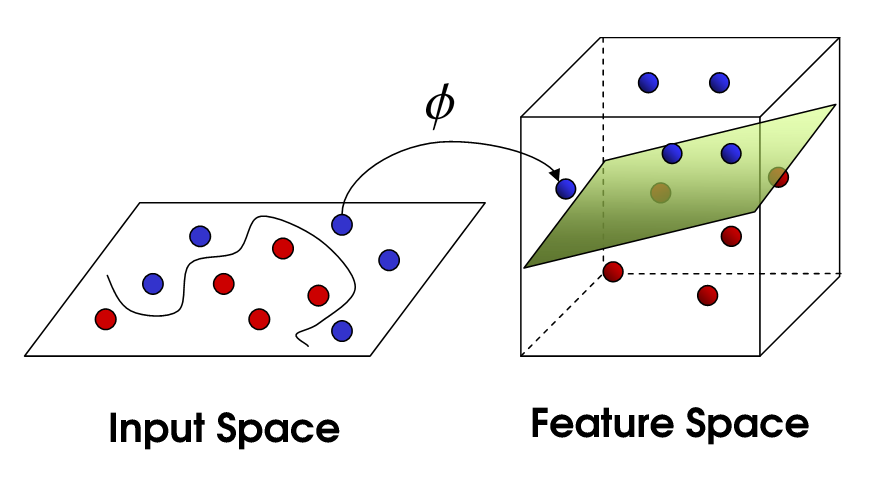
\includegraphics[scale=0.4]{Figures/phi}
    \caption{A visual rendition of the $\phi$ function, mapping samples from the
    input feature space to another feature space of higher dimensionality so that
    they could become linearly separable (from \cite{rtesselli}).}
    \label{fig:phi}
\end{figure}

Given these premises, and a value of $M$ high enough for the mapped samples to
be linearly separable, a kernel machine looks for the optimal linear separator in
$\mathcal{H}$ that corresponds to a non-linear separator in the input space.
To find this optimal separator the kernel machine has to deal with samples of
very high (possibly infinite) dimensionality and this could quickly render the
search for the solution to the optimization problem infeasible or too onerous.
Given that in the problem formulation the function $\phi$ only appears inside
the computation of dot products, values can be calculated by a kernel
function (section~\ref{subsec:kernelfunc}) thus referring to $\mathcal{H}$
only implicitly and avoiding to deal with a high number of dimensions
altogether using what is commonly known as the \emph{kernel trick}.

\subsubsection{Support vector machines}
\label{subsubsec:svm}
Here we will briefly describe one of the most tried kernel machines in the literature. 
\emph{Support Vector Machines} or SVM \cite{Cortes&Vapnik:1995} rest on the principle of structural risk
minimization (Section \ref{subsec:srm}) providing a trade-off between hypotheses
space complexity and the performances in fitting the training data.
It is a binary classifier but can be used to solve multi-class classification
problems with some additional work to combine multiple instances of this binary
classifier.
It is also a linear classifier and can be easily extended to the 
non-linear domain by using it in conjunction with (non-linear) kernel functions.
Given a feature space, this method tries to find the optimal hyperplane that
correctly separates the samples in such space, and separates them in the
most general way that is, maximising the \emph{margin} between each class.
In order to minimize the bound on true error (Section \ref{subsec:srm})
this method uses hypotheses spaces of crescent VC-dimension, to minimize the
VC-confidence while keeping a low empirical error.
There are two main settings in which this algorithm can work: when the data
is linearly separable in its original feature space and when it is not.
In the first case, since the empirical risk is going to be zero, finding the
optimal hyperplane means finding the one that again minimizes the VC-dimension
which in turn is the one that maximizes the margin between the classes i.e.
the minimum distance between the hyperplane and the nearest sample.
Solving this problem equals to solving the following quadratic optimization
problem:

\begin{gather}
    \begin{aligned}
        & min_{\vec{w},b}\frac{1}{2}||\vec{w}||^2 \\
        & \text{s.t. } \forall i \in \{1,\dots, n\} : y_i(\vec{w}\cdot\vec{x_i} + b) - 1 \geq 0 
        \label{eq:lsvm}
    \end{aligned}
\end{gather}

where $\vec{w} \cdot \vec{x} + b$ defines the hyperplane.
Since the margin we are looking to maximize is inversely proportional to the norm
of $\vec{w}$, we want to minimize the latter while the $\frac{1}{2}$ factor stems
from mathematical convenience.
Equation \ref{eq:lsvm} shows the primal form of the problem, whose formulation
has a convex cost function and constraints, hence it can be solved more easily 
switching to its dual form that, given these premises, will have the same
optimal solution.
Thanks to the Kuhn-Tucker theorem we can formulate the dual form using
Lagrange's multipliers:

\begin{gather}
    \underset{\vec{w},b}{\mathrm{min}}\,\underset{\vec{\alpha}\geq 0}{\mathrm{max}}\,L(\vec{w},b,\vec{\alpha})
    \label{eq:ldual}
\end{gather}

where $L$ is the lagrangian function and $\vec{\alpha}$ the multipliers.

\begin{equation}
    L(\vec{w},b,\vec{\alpha}) = \frac{1}{2}||\vec{w}||^2 - \sum_{i=1}^n \alpha_i(y_i(\vec{w}\cdot\vec{x} + b) - 1)
    \label{eq:lagrange}
\end{equation}

The optimal solution of this problem is the saddle point obtained while minimizing
w.r.t. $\vec{w}\text{ and }b$ and maximizing w.r.t. $\vec{\alpha}$.

When reaching this point the gradient of the function $L$ must be null:

\begin{gather}
    \begin{aligned}
        & \frac{\delta L(\vec{w},b,\vec{\alpha})}{\delta\vec{w}} = 0 \iff \vec{w^*} = \sum^{n}_{i=1} y_i\alpha^*_i\vec{x_i}\\
        & \frac{\delta L(\vec{w},b,\vec{\alpha})}{\delta b} = 0 \iff \sum_{i=1}^{n} y_i\alpha^*_i = 0\\
        & \alpha^*_i[y_i(\vec{w^*}\cdot \vec{x_i}+b^*) - 1] = 0,\,i=1,\dots,n
        \label{eq:lagrangedual}
    \end{aligned}
\end{gather}

and this lets us get rid of the primal variables in the lagrangian function since
they can be expressed using the labelled samples and the multipliers hence
reducing the problem to the maximization of $L(\vec{\alpha})$.
Those samples $X_i$ for which the $\alpha^*_i$ are greater than zero are called
support vectors and are the ones closer to the hyperplane, determining the margin,
as can be seen in Figure \ref{fig:slacks}.

The other case, that is when the data is not linearly separable, is solved in a
similar way but with the introduction of \emph{slack variables}, one for each
constraint:

\begin{equation}
    y_i(\vec{w}\cdot\vec{x} + b) \geq 1 - \xi_i
\end{equation}

These variables $\xi_i$, will account for the constraint violations by modifying the cost
function:

\begin{equation}
    \frac{1}{2}||\vec{w}||^2 + C \sum_{i=1}^n \xi_i
\end{equation}

where $C$ is a regularization parameter that will balance the trade-off between
the hypotheses space complexity and the number of non-separable samples.
Recalling the dual form of the previous case after the elimination of the primal
variables from the lagrangian function (Equations \ref{eq:lagrange} and \ref{eq:lagrangedual}),
we can now formulate our problem in the following way:

\begin{gather}
    \begin{aligned}
    & \underset{\vec{\alpha}}{\mathrm{max}} \sum_{i=1}^n \alpha_i - \frac{1}{2} \sum_{i,j=1}^n y_iy_j\alpha_i\alpha_j\vec{x_i}\vec{x_j}\\
    & \text{s.t. } \forall i \in \{1,\dots, n\} : 0 \leq \alpha_i \leq C,\, \sum_{i=1}^n y_i\alpha_i = 0 
    \end{aligned}
\end{gather}

This formulation differs from the previous one in that the dual variables (the $\alpha_i$s)
have $C$ as an upper bound.
The role of the slack variable $\xi_i$ is exemplified in Figure \ref{fig:slacks}.

\begin{figure}[ht]
    \centering
    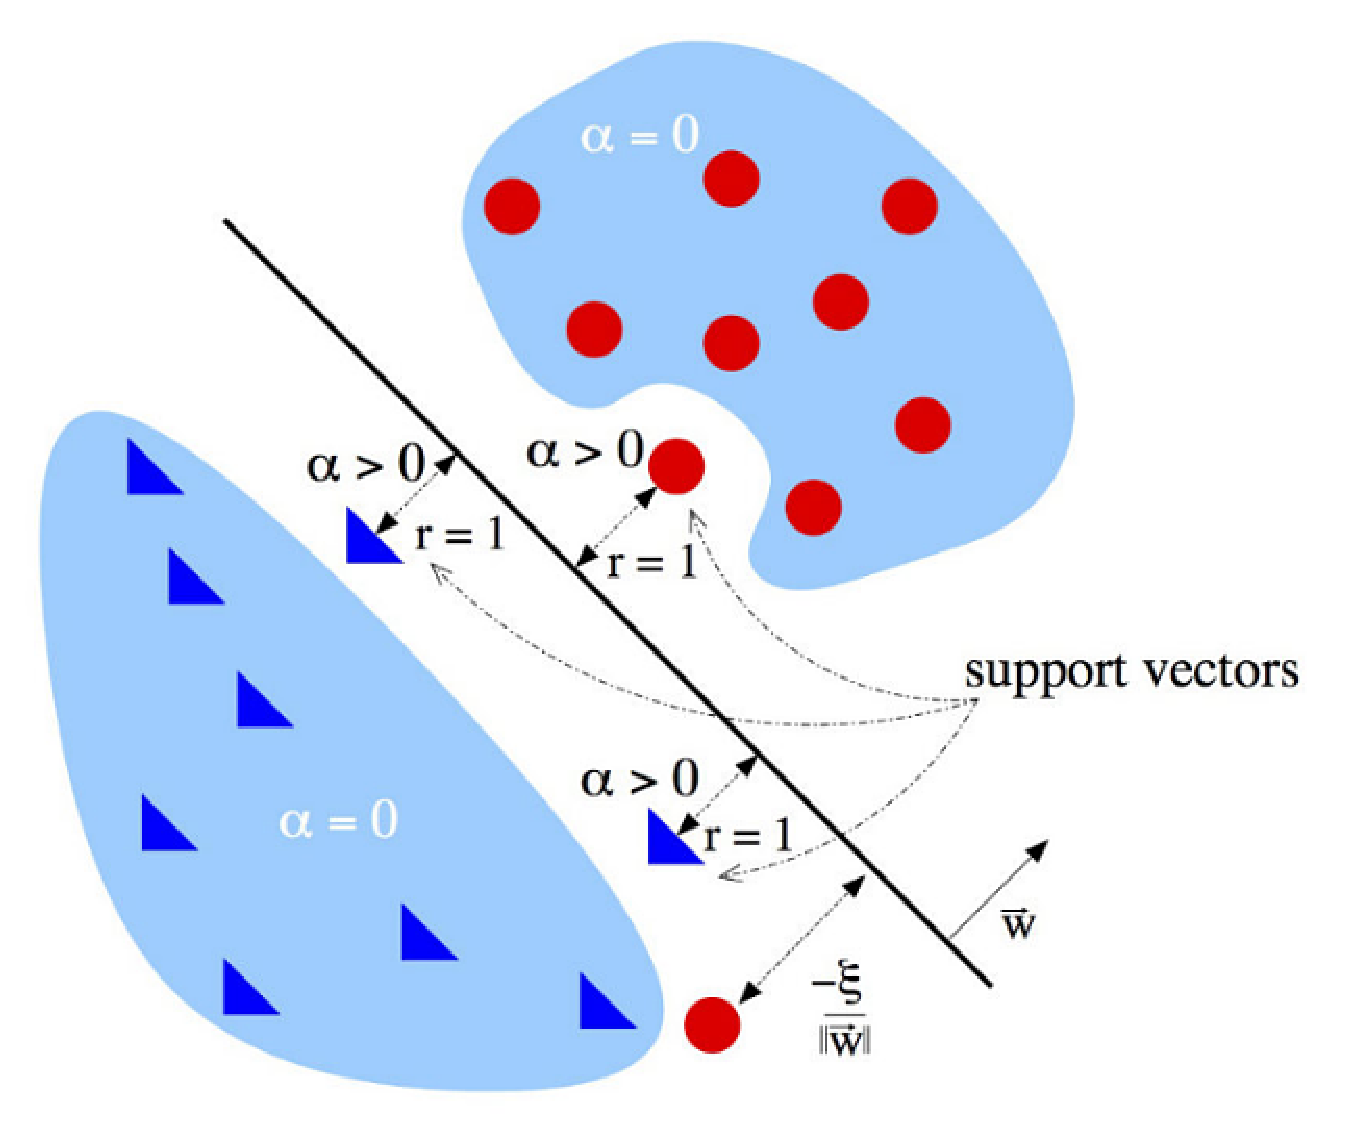
\includegraphics[scale=0.4]{Figures/slacks2}
    \caption{Effect of the introduction of \emph{slack variables} ($\xi$) in the SVM
    formulation variant known as \emph{soft margin} SVM.}
    \label{fig:slacks}
\end{figure}

The above approach has the major drawback that cannot guarantee good performances
in highly non-separable data because of the limitation in the ways an hyperplane
can separate any feature space, i.e. through dichotomies.
A remedy to this fact is to use the technique exposed in Section \ref{subsec:kmachines}
while maintaining the same formulation explained above where the dot product between
the samples in the (mapped) feature space is substituted with the kernel value on the
same samples.
The effects of this technique on the classification task is visible in Figure \ref{fig:kernsvm}.

\begin{figure}[ht]
    \centering
    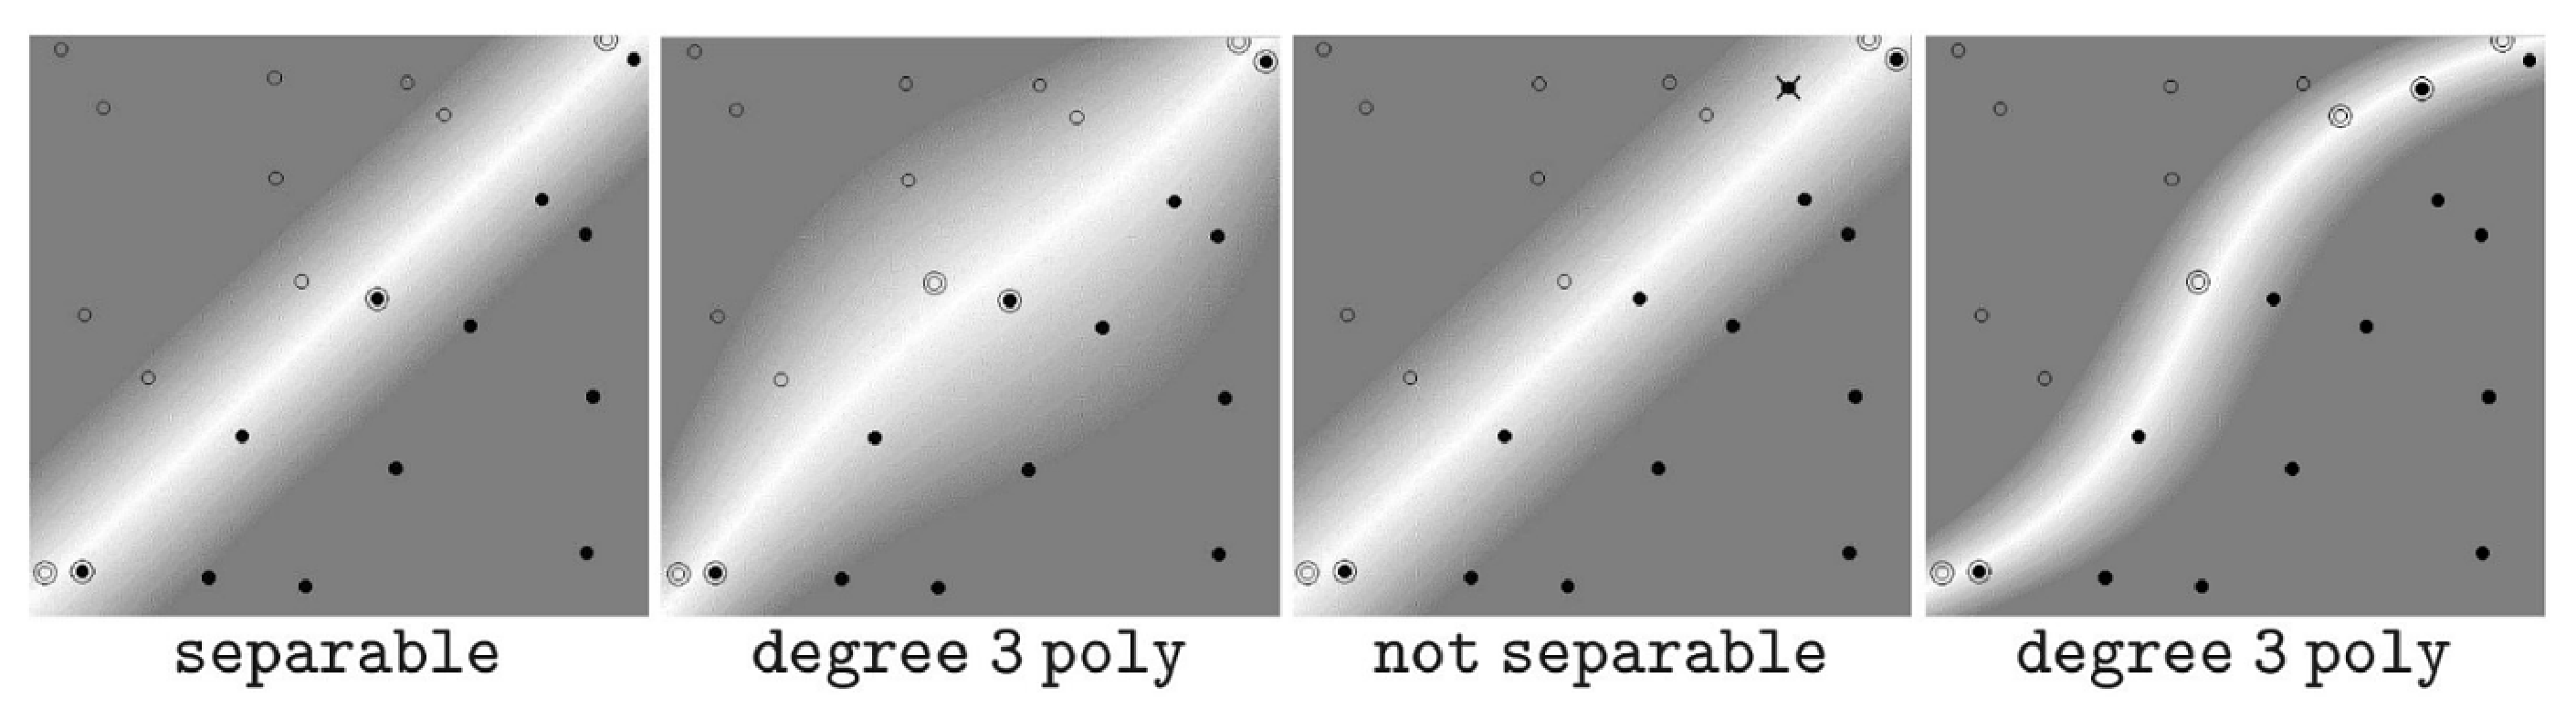
\includegraphics[scale=0.3]{Figures/kernsvm}
    \caption{Different effects on the decision surfaces generated on the input
        feature space without (first and third pictures) and with kernel (second and last pictures)
        in the two cases where data is linearly (first two pictures) and non-linearly separable (last two pictures)
        [ref lecture slides].}
    \label{fig:kernsvm}
\end{figure}

%----------------------------------------------------------------------------------------

\section{Kernels for structured data}
\label{sec:graphkernels}

In the previous section we introduced the theoretical foundations behind kernel
functions and the related learning methods.
The kernel learning approach is certainly convenient, the user needs to concentrate
its effort on the selection or design of the right kernel function for the problem
at hand, then couple it with one of the available general-purpose learning algorithms to
get a full-fledged learning method.
That being said, it is clear that in this scenario the kernel function is the
component responsible for the main source of bias.
Nowadays a number of different kernel functions are available with varying degree
of complexity in order to deal with a variety of problems, most of which has data
represented in vectorial form.
The rise of problems where data is naturally better represented with a
structured form (Section \ref{subsubsec:examples}) has rendered necessary the
study of new methods to tackle them.
One way of working with structured data could be to actually get rid of the structure
deriving an \emph{ad-hoc} vectorial representation, in what is called a
\emph{structure-based} approach.
This method is expensive and cumbersome since it forces the user to have a strong
knowledge of the task domain and to re-develop a new vectorial representation
for each task that she may encounter.

A more effective approach would be to adapt the methods to work directly on
structured data, and in this regard kernel methods are a good fit since the
decoupling between the kernel function and the kernel machine leaves the
only contact point between the data and the method in the function itself.
These methods maps the sample instances into high dimensional vectors and do it
in a general way without any knowledge of the underlying data beside its structure.
Furthermore this mapping is done implicitly meaning that they also have an
advantage from a computational standpoint.

Designing such kernel functions that can deal with structured data is a process
that has to balance between designing functions that are expressive enough to
produce some learning and the computational efficiency that it is required in
order to effectively perform the learning process.
As an example of this trade-off consider a kernel on graphs that counts all the
matching subgraphs between two input graphs.
This is certainly one of the most expressive possible kernels if not the most expressive
at all.
Even if such enumeration would exist, the kernel would still need to solve the
subgraph isomorphism problem several times, but that is clearly infeasible since subgraph
isomorphism is NP-hard.
Algorithmic complexity for a kernel function is a major point since the kernel has
to be computed for each pair of samples, rendering even a quadratic complexity
a hindering factor for its application.

A theoretically grounded way to design efficient and effective kernel functions for
structured data has been proposed by Haussler \cite{haussler99convolution} and
it is explained in the next section.
The main concept behind his work is that we need to restrict the number and type
of features considered for each structure.
Again, the choice of the substructures that would become features deeply affects
the learning outcome and is one of the major sources of bias in the whole learning
process, possibly leading to greatly differing performances according to different
datasets.
For what concern the scope of this thesis we will see in the following sections
some examples of kernels defined on trees and on graphs, all of which are instances
of the framework proposed by Haussler.

\subsection{The framework: convolution kernels}
\label{subsec:convolution}
Haussler's work \cite{haussler99convolution} main result is the \emph{R-convolution} framework,
a method for defining positive definite kernel functions on any object provided that a
positive semidefinite kernel for some decomposition of that object is available.
To give a brief formalization of the main idea, let $\mathcal{X}$ be a space of 
objects such that $x \in \mathcal{X}$ is associated with a finite subset
$\mathcal{X'_\mathit{x}}$ of some space $\mathcal{X'}$.
Assuming that: a kernel $k: \mathcal{X'}\times \mathcal{X'} \to \mathbb{R}$ is
defined and a \emph{finite} relation $R \subseteq \mathcal{X'}^D \times \mathcal{X'}$
is defined, we can now define an $R-convolution$ kernel:

\begin{equation}
    K(x,y) = \sum_{(x'_1,\dots,x'_n,x) \in R} \Bigg(\sum_{(y'_1,\dots,y'_n,y) \in R}
    \prod_{i=1}^D k(x'_i,y'_i)\Bigg)
\end{equation}

that, with the commonly used formulation with $D=1$ becomes:

\begin{equation}
    K(x,y) = \sum_{(x',x) \in R} \sum_{(y',y) \in R} k(x'_i,y'_i)
\end{equation}

Haussler was able to demonstrate the positive semi-definiteness of any kernel $K$
thusly defined, provided that $k$ is also positive semi-definite.

This work has later been extended and generalized \cite{Shin2010} with the introduction
of the \emph{mapping} kernel of which the \emph{R-convolution} kernel is a corollary.
This more general framework defines a mapping set
$M_{x,y} \subseteq \mathcal{X'_\mathit{x}} \times \mathcal{X'_\mathit{y}}$ and a \emph{base kernel} $k$ on it
that will hence consider only a subset of the entire cross product $\mathcal{X'_\mathit{x}} \times \mathcal{X'_\mathit{y}}$.
With these premises, a mapping kernel is defined as:
    
\begin{equation}
    K(x,y) = \sum_{(x',y') \in M_{x,y}} k(x',y')
\end{equation}

The positive semi-definiteness of the kernel $K$ is guaranteed only if the
mapping $\{M_{x,y}|x,y \in \mathcal{X}\}$ is transitive.
In the following sections we will analyse some of the latest contributions in terms
of kernel on structured data namely tree kernels and graph kernels.

\subsection{Kernels for trees}
This family of kernels stems directly from the convolution kernel and each one
works by defining a different decomposition for the input tree.

\subsubsection{Subtree kernel}
\label{subsubsec:st}
The feature space of this kernel is composed of all the proper subtrees of the
input tree.
Let $X$ and $Y$ be two trees, the  subtree kernel is defined as:
\begin{equation}
    K_{ST}(X,Y) = \sum_{x \in X} \sum_{y \in Y} \delta(x,y)w_x =
    \sum_{s \in \mathcal{A}^*} h_s(X)h_s(Y)w_s
\end{equation}

where $x$ and $y$ are proper subtrees of $X$ and $Y$ respectively, $w_x$ is the 
weight associated with the tree $x$, $\mathcal{A}^*$ is the set of all the possible
subtrees, $h_s(X)$ counts the frequency with which $s$ appears in $X$ and
$\delta$ is the Kronecker's delta function, a function that evaluates to 1 if its
arguments matches, 0 otherwise.
The complexity of this formulation is indeed quadratic but in practice it can be
lowered to $O(nlogn)$, $n$ being the maximum number of nodes in either $X$ or $Y$,
using suffix trees \cite{viswanathan04fastkernels}.

\subsubsection{Augmented subtree kernel}
A more discriminative version of the previous kernel is the \emph{augmented} version
which extends the feature space of the subtree kernel with new features.
Usually adding more feature has an impact on the computational side of a kernel,
in \cite{dasanmartino2015exploiting} however an extension called ST+ kernel has been proposed with
only a modest increment in computational time.
Given a tree $T$, this kernel considers at most $\rho(v)h + 1$ features for any
$v \in V_T$ which are:
\begin{itemize}
    \item the proper subtree rooted at $v$, $\overset{v}{\triangle}$;
    \item for every $j^{th}$ child of $v$, $ch_v[j]$, and for every $l\text{ s.t. }0 \leq l < h$,
        the subtree of $T$ composed by:
        \begin{itemize}
            \item $v$ as root,
            \item $\overset{ch_v[j]}{\triangle}$,
            \item $T_{l-1}(ch_v[i],T) \forall i \in children(v), i \ne j$.
        \end{itemize}
\end{itemize}

An example of feature extraction is given in Figure \ref{fig:featext}.

\begin{figure}[ht]
    \centering
    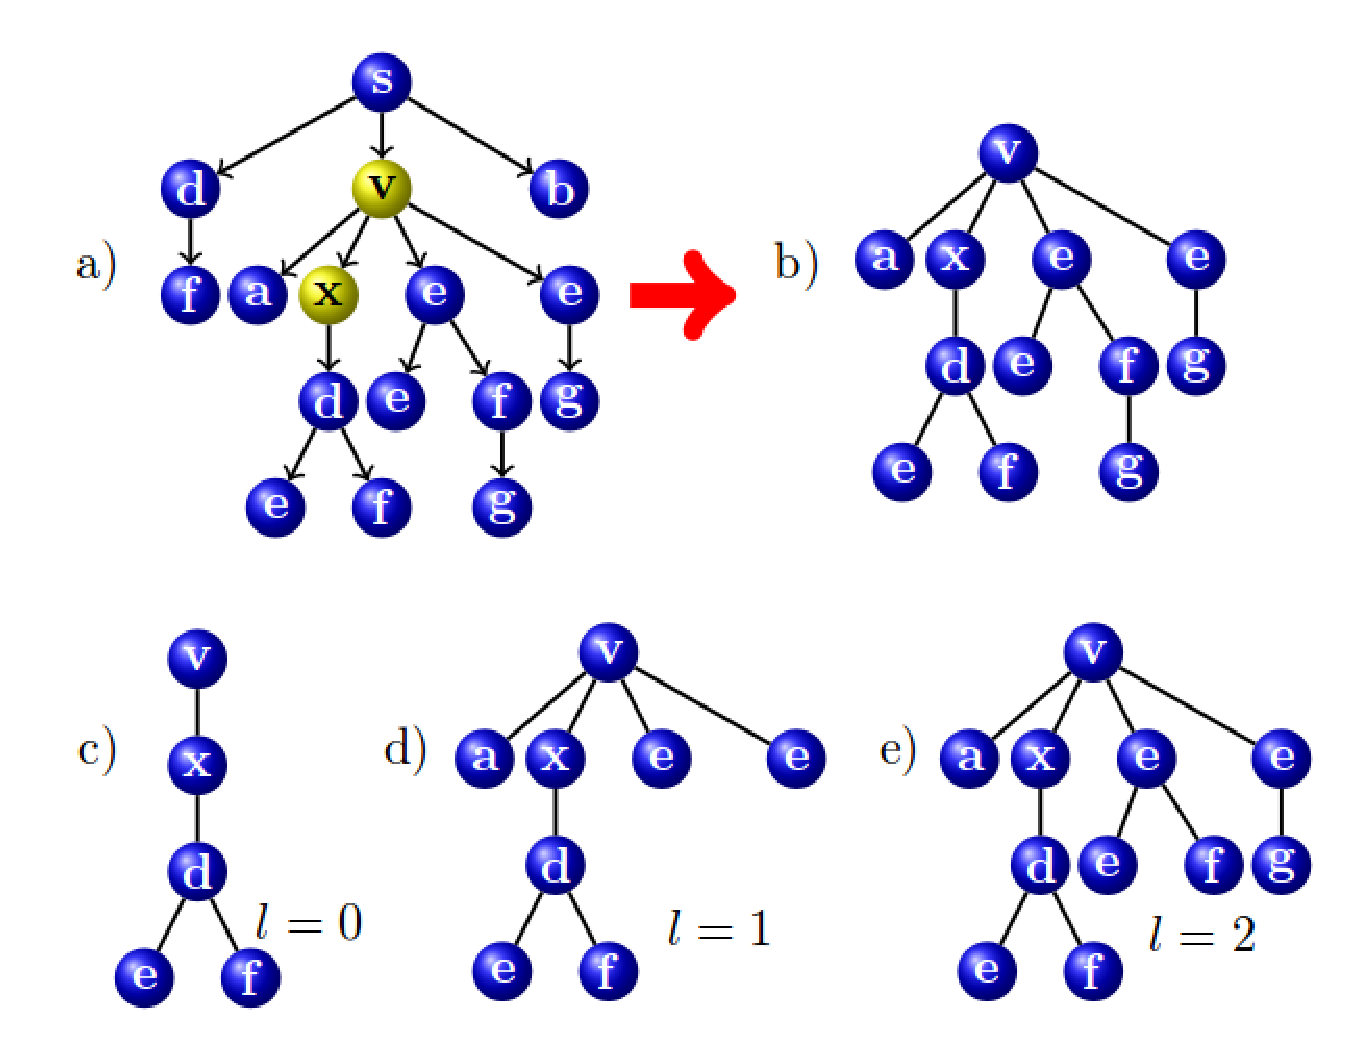
\includegraphics[scale=0.4]{Figures/featext}
    \caption{Feature space representation related to the kernel ST+ for an example
    tree: a) the input tree; b) the proper subtree rooted at the node labelled as $v$;
    c)-e) given the child $x$ of $v$, the features related to visits limited to $l$ levels (from \cite{dasanmartino2015exploiting}).} 
    \label{fig:featext}
\end{figure}

The formulation of this kernel is the following:

\begin{equation}
    K_{ST+}(T_1, T_2) = \sum_{s=1}^m h_s(T_1)h_s(T_2)
\end{equation}

where $m$ is the number of distinct trees corresponding to ST+ features, extracted
from a finite set of trees, and $h_s(T)$ the number of times the feature $t_s$
appears in $T$.

The proposed implementation in \cite{dasanmartino2015exploiting} has a complexity of
$O(Hh^2\rho^2log\rho)$ with $h$ and $H$ being the limit
of the tree visit and the number of nodes of that tree respectively.

\subsection{Kernels for graphs}
\label{subsec:graphk}

As previously mentioned, defining kernels on graph is a challenging task, mainly
because of the need to balance the trade-off between the expressiveness of the
feature space and the computational effort needed for feature extraction and
kernel calculation.
Expressive kernels are usually well performing in terms of predictive power but
are also typically more expensive to compute.
On the other hand a less discriminative kernel is usually easier to calculate
at the expenses of some learning power.
To further explain this point, consider the class of kernels that are able to
distinguish between all the (non-isomorphic) graphs in the feature space.
Being able to distinguishing between two non-isomorphic graphs that belongs to two
different classes is essential for any machine learning approach.
However, computing such kernel in an efficient way would equals to solve the
graph isomorphism problem in a similarly efficient way and this is not the case
since at the moment there are no polynomial time algorithms for solving the graph isomorphism problem.
Another interesting group of kernels is the one that given a graph $X$, it decomposes
it into the set of its subgraphs and maps it to a set of features $\phi_h$ that, for
each graph $h$ measure how many subgraphs of $X$ are isomorphic to $h$.
Again this class of kernels has to deal with the solution of the same NP-hard
problem explained above, so probably no such efficient kernel exists.

Recent research has focused on the study and development of less expressive
kernels that have the major advantage of being computable in polynomial time.
In the following sections we will briefly discuss the kernels that falls in the
scope of the present thesis, and give an overview of the recent improvements that
have been proposed in the literature.

\subsubsection{ODD kernels}
\label{subsubsec:odd}

Before the introduction of the ODD kernel framework, a number of graph kernels
could already be found in literature, such as the \emph{random walk kernels} \cite{Gaertner04mlj},
the \emph{subtree pattern kernel} \cite{ramon03graphkernels}, and the \emph{shortest path kernel}
\cite{borgwardt05graphkernel}, but they remained computationally very onerous, with
the first family having polynomial complexity only on undirected graphs, the second one
having exponential complexity and the last one being more than quadratic.
The \emph{ODD kernel framework} proposed in \cite{DBLP:conf/sdm/MartinoNS12} aims
to be a kernel framework that can be instantiated with the right trade-off between
expressiveness and efficiency for different tasks.
The original work presents an instantiation with the ST kernel, while another
recent work \cite{dasanmartino2015exploiting} instances the framework to an adaption
of the ST+ kernel.

The Ordered Decomposition DAG Kernels framework (ODDK) basically decomposes the
graphs in a set of simpler trees, where it is easier to compute the isomorphism
using efficient tree kernels.
The framework consists of these steps:

\begin{enumerate}
    \item the input graph $g$ is mapped into a multiset of decomposition DAGs\\
        $\{DD_g^{v_i}|v_i \in V_g\}$; $DD_g^{v_i}$ is obtained from its root $v_i$
        and the edges that appear in the shortest paths from $v_i$ to any other node
        $v_j \in V_g$;
    \item a strict partial order on the vertices of the DAG has to be defined
        to make an unique representation of the subtrees possible.
    \item each Ordered Decomposition DAG $ODD_g^{v_i}$ thus obtained that is, each
        decomposition DAG with the nodes ordered according to the partial
        order relation defined above, is then mapped into
        one or more trees $T(v_i,ODD_g^{v_i})$, where $T(\cdot,\cdot)$ is the function
        that returns the tree resulting from the tree visit on $ODD_g^{v_i}$ starting
        from node $v_i$, and the kernel between two graphs $g_1$ and $g_2$ is
        defined as:
        \begin{equation}
            ODDK(g_1,g_2) = \underset{OD_2 \in ODD_{g2}}{\underset{OD_1 \in ODD_{g1}}{\sum}}
            \sum_{j=1}^h\sum_{l=1}^h
            \underset{v_2 \in V_{OD_2}}{\underset{v_1 \in V_{OD_1}}{\sum}}
            C(r(T_j(v_1,OD_1),r(T_l(v_2,OD_2)))
        \end{equation}
        where $C$ is the function defined by the chosen tree kernel.
\end{enumerate}

Considering the instantiation of the framework with the ST kernel and limiting
the size of the tree-visits $T_j(v_1)$, with the $h$ parameter that regulates the
maximum height of the considered substructures, and by assuming $\rho$ constant
the time complexity of $ODDK$ with ST features is $O(|V_g|log|V_g|)$.

\subsubsection{Fast subtree kernels}
\label{subsubsec:fs}
The fast subtree kernel \cite{NIPS2009_3813} belongs to family of kernels defined
as instances of the Weisfeiler-Lehman kernel framework which bases its discriminative
power on the Weisfeiler-Lehman test of isomorphism.
The main idea behind this framework is that every graph can be represented as
a sequence of graphs, each one being generated from the previous one through
a new labeling function that encapsulates the isomorphism test.
Given a graph $X = (V,E,L)$, this sequence can be formally defined as:

\[\{X_0,X_1,\dots,X_h\} = \{(V,E,L_0),(V,E,L_1),\dots,(V,E,L_h)\}\]

where $X_0 = X$, $L_0 = L$ and $L_i$ is represents the relabeling of the graph
$X_{i-1}$ obtained applying the Weisfeiler-Lehman test.

Let $k$ be a positive semidefinite kernel for graphs the Weisfeiler-Lehman kernel
framework can be formulated as:

\begin{equation}
    K_{WL}^h(X,Y) = k(X_0,Y_0) + k(X_1,Y_1) + \dots + k(X_h,Y_h)
    \label{eq:fs}
\end{equation}

A first instance of this framework is the \emph{Weisfeiler-Lehman subtree kernel}
($WL$) which considers all the subtree patterns up to height $h$ and checks whether the
neighbourhoods of two nodes match exactly.
To define this kernel it is sufficient to define the base kernel for Equation
\ref{eq:fs} as:

\begin{equation}
    k(X,Y) = \sum_{x \in V(X)}\sum_{y \in V(Y)} \delta(L(x),L(y))
    \label{eq:wl}
\end{equation}

where $\delta$ is again the Kronecker's function.

With the base kernel defined in Equation \ref{eq:wl}, $K_{WL}^h$ becomes the
kernel defined in \cite{NIPS2009_3813}.

\subsection{Latest improvements on graph kernel methods}
\label{subsec:kernel}
In the recent years a number of improvement over the above mentioned kernel approaches
have been proposed, mainly to try to improve the expressiveness of the feature
spaces without incurring in major computational drawbacks.
Among the others, and mainly because inside the scope of this thesis we will
mention in no particular order:
\begin{itemize}
    \item the addition of contextual information \cite{Navarin2015},
    \item the extension of the $ODD_{ST}$ kernel to employ an MKL approach,
    \item the extension and generalization of the Weisfeiler-Lehman framework \cite{SanMartino2014}.
\end{itemize}

The next section will give a brief overview of the first point while in section
\ref{subsec:gmkl} we will delve a bit more in detail in the MKL approach
with respect to graph kernel learning.

\subsubsection{Kernels with contextual information}
\label{subsec:context}

The kernels described in the previous section try to approximate complex
structures by the means of decomposing them in simpler substructures on which
define a measure of similarity.
Even though they employ different type of substructures, they have in general
similar predictive performances.
A recently proposed work \cite{Navarin2015} on graph kernels, aims to improve local
feature expressiveness by enriching the feature space with contextual information,
that is, a description of the topology of the graph around the extracted feature.
The cited work proposes an extension of the $ODD_{ST}$ kernel, derived from
\cite{rtesselli} where extensions of the $ODD_{ST+}$ kernel ($TCK_{ST+})$ and of the $WL$
kernel ($WLC$) are proposed.
In this way an increase of discriminative power is expected, since two identical
features need also to appear in the same context within two graphs to match.
Therefore a feature contribution is built up by the contribution determined by
its contexts. To express it more formally, given a graph $g$ and a feature $f$
the following property holds from \cite{Navarin2015}:

\begin{equation}
    \phi_f(g) = \sum_{c \in Contexts_g(f)} \phi_{f\circ c}(g)
\end{equation}

where $\phi_f(g)$ is the frequency of the feature $f$ in the RKHS of the original
kernel and $\phi_f\circ c(g)$ is the frequency of the it appearing within the
context $c$.

Given the parent-child relationship between contexts and features, it is
straightforward to see that they can share the same representation, i.e. the
context is a substructure of the graph that contains the feature.
This leads to the useful facts that context can be feature themselves and that to
compute contextualized features it suffices to combine features with other
features representing contexts.
The Tree Context Kernel can thus be defined as:

\begin{gather}
    \begin{aligned}
        TCK(G_1,G_2) &= \underset{v_2 \in V_{G_2}}{\underset{v_1 \in V_{G_1}}{\sum}}
        \sum_{i=1}^h\sum_{j=1}^h
        ~[\delta(T_i(v_1,G_1),T_j(v_2,G_2))\\
            &+\underset{\overset{u_2}{\triangle} \in T_i(v_2,G_2)}{\underset{\overset{u_1}{\triangle} \in T_i(v_1,G_1)}{\sum}}
        \delta(\overset{u_1}{\triangle},\overset{u_2}{\triangle})
    \sum_{l=1}^{\rho(u_1)} C_{ST}(ch_l(u_1),ch_l(u_2))]
    \end{aligned}
\end{gather}

%where:
%
%\begin{equation*}
%    C_{ST}(v_1,v_2) = 
%        \begin{cases}
%            \lambda \cdot K_L(v_1,v_2) & \text{if } v_1 \text{ and } v_2 \text{ are leaves} \\
%            \lambda \cdot K_L(v_1,v_2)\,\prod_{j=1}^{\rho(v_1)} C_{ST}(ch_j(v_1),ch_j(v_2)) & \text{if } \rho(v_1)=\rho(v_2) \\
%            0 & \text{ otherwise}
%        \end{cases}
%\end{equation*}

where $\delta$ is the Kronecker's function, $h$ is the user defined depth limit of 
the tree-visit and $C_{ST}$ is the function related to the ST kernel (see Section \ref{subsubsec:st}) that counts the common
subtrees of the two trees rooted at $v_1$ and $v_2$.

In more simple terms the kernel will score a match in the following cases:
\begin{itemize}
    \item both $v_1$ and $v_2$ are root nodes of the tree visit, i.e. $u_1 = v_1$ and $u_2 = v_2$
    \item $v_1$ and $v_2$ appear within the same context in both the trees
\end{itemize}

This kernel is provably positive semidefinite because it is a combination of positive
semidefinite kernels (see the end of Section \ref{subsec:convolution}).

\section{Multiple kernel learning}
\label{subsec:mkl}
Multiple Kernel Learning aims to enhance the accuracy of a target kernel machine
combining kernels derived from multiple sources in a data-driven way.
The rationale behind this idea is similar to the one behind classifier combinations.
Instead of deciding a priori which kernel to use, it is better to devise an
algorithm that can either choose for us or better, learn a combination of the
possible choices.

Hence MKL can be used to mitigate the bias deriving from a single kernel choice
or to combine different source of information that rely on different data representation
thus requiring a number of different kernels.

Furthermore it relieves the final user from the often arduous task of designing
a strong kernel by allowing her to implement a number of more ``weak'' kernels
that can work in combination to perform the learning task.

The available methods in the literature can be summarily divided in two categories
\cite{journals/jmlr/GonenA11}: on one hand \emph{fixed rule} algorithms which as the name implies apply some fixed
rule or heuristic to determine the combination parameters, thus being able to scale
well with respect to the number of kernels but whose effectiveness is bounded by
the effectiveness of the rule on the domain being considered,
on the other hand, \emph{optimization based} approaches solve an optimization
problem to derive their combination parameters.

There are two fundamental ways to use the MKL approach: combine a small set of 
relatively strong and carefully designed kernels, a method which has shown no
significant improvement over a simple combination like the averaging of the kernels;
then the converse, combine a large set of weak kernels aiming at boosting their
individual performances exploiting a data driven rather than an expert driven
approach.

In the following section we will give an overview of the MKL implementation
that we chose for the present work.

\subsection{EasyMKL}
\label{subsec:easymkl}

The method proposed in \cite{aiolli2015easymkl} focuses on the linear positive combination
parameters version of MKL which can be formulated as

\begin{equation}
    K = \sum_{r=1}^R \eta_rK_r,\, \eta_r \geq 0
    \label{eq:easymkl}
\end{equation}

The goal is to learn a vector of coefficients $\vec{\eta}=\{\eta_r\}_{1\leq r \leq R}$ that will form the
combined kernel according to Equation \ref{eq:easymkl}.
The proposed algorithm can be ascribed to the category of optimization based
techniques since in it requires the solution of an optimization problem whose
formulation follows:

\begin{equation}
    \underset{\vec{\eta}:||\vec{\eta}||=1}{\mathrm{max}}\underset{\gamma \in \hat{\Gamma}}{\mathrm{min}}(1-\Lambda)\gamma^\top\hat{Y}\Big(\boldsymbol{\sum_r^R \eta_r\hat{K_r}}\Big)\hat{Y}\gamma+\Lambda||\gamma||^2_2
    \label{eq:easymin}
\end{equation}

where $\hat{K_r}\text{ and }\hat{Y}$ are the weak kernel computed on the training samples
and the training labels respectively, $\Lambda \in \{0,1\}$ is the regularization
parameter and $\gamma \in \hat{\Gamma}$ is the probability distribution over the set of positive and
negative training samples, $\hat{\Gamma}$ being the domain of probability distributions defined as:
\[ \hat{\Gamma} = \Big\{ \gamma \in \mathbb{R}^l_+ | \sum_{i \in \oplus} \gamma_i = 1, \sum_{i \in \ominus} \gamma_i = 1 \Big\} \]

This problem has a formulation similar to the one of the \emph{Kernel Optimization of the
Margin Distribution} algorithm (KOMD) \cite{Aiolli2008} where the kernel has been
substituted with the sum of the weak input kernels with the important implication
that the space requirements remain linear w.r.t. $R$.

In the margin maximization step of the algorithm, the $\Lambda$ parameter
has two critical points: when $\Lambda = 0$ there is no regularization so the
problem reduces to a hard margin SVM; when $\Lambda = 1$ the optimal solution is
the squared distance between the positive and negative centroids in the feature
space.
EasyMKL is a non-sparse MKL method because it employs the 2-norm in its regularization
term, hence working best in conjunction with orthogonalized kernels while remaining
resilient w.r.t. noise and duplicate features \cite{KloBreSonZie11}.

\subsection{Multiple kernel learning on graphs}
\label{subsec:gmkl}
A recent work \cite{gmkl} has managed to integrate the algorithm explained in the
previous section with the work on graph kernels conducted in \cite{DBLP:conf/sdm/MartinoNS12}.

The technique proposed in the paper aims to find a generalizable way of constructing
orthogonalized kernels starting from a single feature space, by the means of 
dividing the features in independent sets according to some strategy.

The work in \cite{gmkl} proposes a simple yet theoretically backed strategy that is,
the subdivision of the feature space of the $ODDK_{ST}$ kernel according to the
size of the features.
Given the inherent hierarchical structure of the tree features, dividing them by
height ensures that no two dependent features ends up in the same set.
Every set composed in this way is then used as a separate feature space to compute
a separate kernel and the whole list becomes the input for the EasyMKL algorithm.
An important point that emerges from this work is that, by using the MKL approach
in combination with an orthogonal partitioning of the feature space, it is possible
to achieve a reduction in the number of hyper-parameters to validate.
This latter point in particular it is a considerable addition to our proposed
methodology as explained in Section \ref{subsec:features}.

%----------------------------------------------------------------------------------------

% vim: spell spelllang=en_gb
